\documentclass{article}
\usepackage {tikz}
\usetikzlibrary {positioning}
\begin{document}

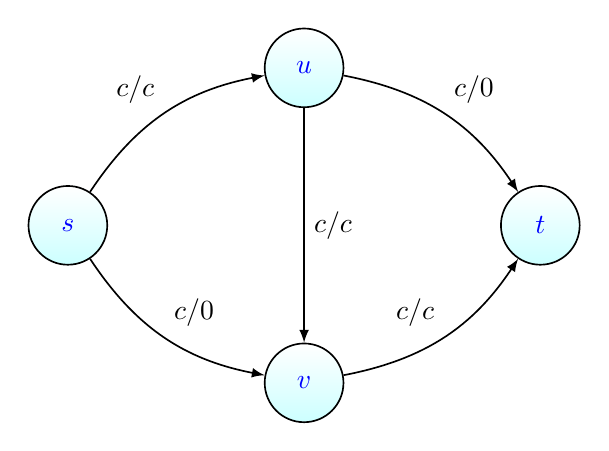
\begin{tikzpicture}[-latex, auto, semithick,
vertex/.style = { circle, top color = white, bottom color = cyan!20, draw, text = blue, minimum width = 
1cm},
arc_ori/.style = { color = black },
arc_res/.style = { color = red }]
\node[vertex] (s) at (-3,0) {$s$};
\node[vertex] (t) at (3,0){$t$};
\node[vertex] (u) at (0,2){$u$};
\node[vertex] (v) at (0, -2){$v$};
\path[arc_ori](s) edge[bend left = 0.8cm] node {$c/c$}(u);
\path[arc_ori](s) edge[bend right = 0.8cm] node {$c/0$}(v);
\path[arc_ori](u) edge node {$c/c$}(v);
\path[arc_ori](u) edge[bend left = 0.8cm] node {$c/0$}(t);
\path[arc_ori](v) edge[bend right = 0.8cm] node {$c/c$}(t);
\end{tikzpicture}

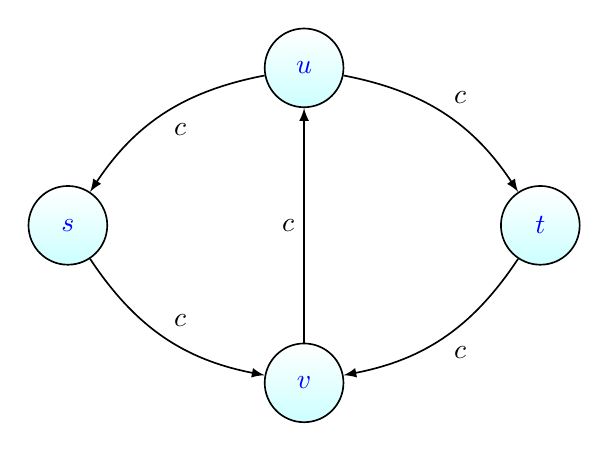
\begin{tikzpicture}[-latex, auto, semithick,
vertex/.style = { circle, top color = white, bottom color = cyan!20, draw, text = blue, minimum width = 
1cm},
arc_ori/.style = { color = black },
arc_res/.style = { color = red }]
\node[vertex] (s) at (-3,0) {$s$};
\node[vertex] (t) at (3,0){$t$};
\node[vertex] (u) at (0,2){$u$};
\node[vertex] (v) at (0, -2){$v$};
\path[arc_ori](u) edge[bend right = 0.8cm] node {$c$}(s);
\path[arc_ori](s) edge[bend right = 0.8cm] node {$c$}(v);
\path[arc_ori](v) edge node {$c$}(u);
\path[arc_ori](u) edge[bend left = 0.8cm] node {$c$}(t);
\path[arc_ori](t) edge[bend left = 0.8cm] node {$c$}(v);
\end{tikzpicture}

\end{document}